\section{大坑:假如明天你突然丢失电脑所有数据怎么办?——如何备份资料}

\begin{figure}[H]
    \begin{tabular}{rl}
        
\includegraphics[width=0.5\columnwidth]{author-folder/Kai.Wu/backup1.jpg} &
        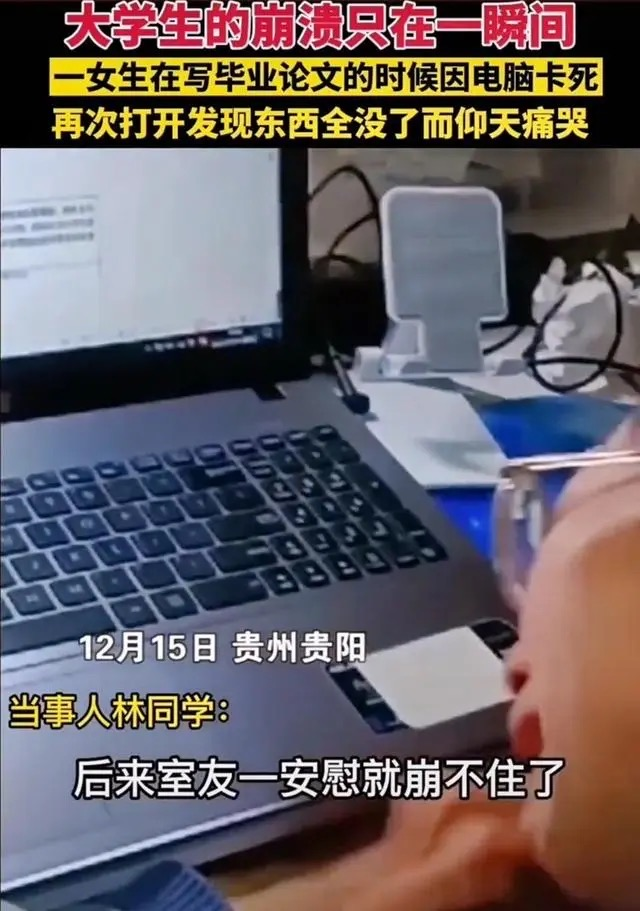
\includegraphics[width=0.4\columnwidth]{author-folder/Kai.Wu/backup2.jpg}
    \end{tabular}
    \caption{\href{https://baijiahao.baidu.com/s?id=1719578217211021768}{链接:贵阳一女大学生8000字毕业论文保存失败崩溃大哭}}
\end{figure}

绝大部分同学本科就买了自己的电脑。虽然自己的各种作业资料,到现在博士阶段的研究数据、论文,全部就只存放在这一台电脑里,但并没有足够意识到自己电脑的重要,和保存在电脑里信息的脆弱。每年,都会有如上图的事情发生,给当事人带来上新闻被全国人民笑话的沉重打击。

丢失一篇正在写的论文,其实是小事,毕竟研究资料全部都在。上面新闻的当事人,其实也就用了几天时间就重新写好了论文。但那些万年不动、又极其重要的资料,又是绝对安全的吗?

想象一下,假如
\begin{itemize}
    \item 你某天手一滑,电脑摔倒地上,再也开不了机,硬盘也没法恢复
    \item 头昏脑涨的一天,你接了一杯咖啡,一不注意,咖啡撒在了电脑上,瞬间短路,电脑滋滋冒油
    \item 你不慎点击了一个链接,中了勒索病毒;或者,西浦内网被网络攻击攻陷,所有电脑中勒索病毒。你的所有文件被加密封锁。
    \item 你把电脑带出去办公或者采集数据,整个电脑直接被偷走
    \item 你过年回家,在路上,背包或者行李箱被人偷走了或者拿错了
    \item 无恶意,但万一,西浦着火了,西浦进水了(MB的5楼一下大雨就漏水),西浦楼塌了,撤离的时候你根本来不及拿电脑
\end{itemize}


\begin{figure}[H]
    \centering
    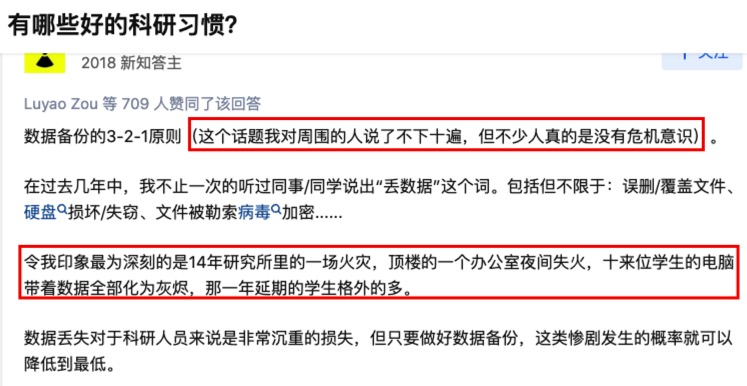
\includegraphics[width=0.8\columnwidth]{author-folder/Kai.Wu/backup_zhihu.jpg}
    \caption{\url{https://www.zhihu.com/question/394796969/answer/1501840215}}
\end{figure}

这些情况,单个可能很罕见,但所有可能性加起来,再乘以3到4年时间,至少发生一次的概率并不小。如果发生,你的博士进度会被耽误多久,你的青春又会被耽误多久呢。

只有一份的数据是非常脆弱的。现在思考一下,你赖以生存的电脑、数据、论文,是否只存了一份?如果是,请立即把屁股从椅子上挪起来,去厕所洗把脸,问问自己都是成年人了,怎么心这么大,然后开始看下面的攻略。

\subsection{理论:321原则}

「3-2-1 原则」是商业公司通用的数据备份金方法,具体内容是:
\begin{itemize}
    \item 3:存储 3 份完整文件,一份原件加上两份拷贝。
    \item 2:将文件起码保持在两种不同的介质上。
    \item 1:将一份拷贝保存在异地。
\end{itemize}

所谓的「介质」,是指内置硬盘、移动硬盘、U盘、网盘等不同的存储介质。说起来好像很麻烦,但对我们来说最简单的实践是:原件保存在内置硬盘,将两份拷贝分别存到移动硬盘和网盘,就同时达成了三条要求。这时,你回过头去看一下我上面列举的所有可能的灾难性问题(甚至即使是网盘公司突然倒闭),都能做到游刃有余,不影响你的科研!

\subsection{实践}

到动手准备的环节了。首先根据你手里的资源,决定你要备份的范围。最土豪的情况,你可以把整个电脑做一个本地备份 + 云端网盘备份,但很多时候,要么网盘容量很小,要么移动硬盘容量不够,要么网速太慢把太多资料传网上很慢,所以先划定你的备份范围。

\begin{itemize}
    \item 最经济的方案:只备份最重要的文件。例如:论文、科研资料、CV、电脑桌面,等等。网盘实时备份+移动硬盘定期备份。对移动硬盘和网盘容量要求都很小。
    \item 最高效的方案:整个电脑(包括最重要的数据)本地备份;最重要的科研、论文等加一分网盘实时备份。这需要一块比你电脑硬盘更大的移动硬盘(不贵),加正常容量(10个G左右)的网盘。
    \item \sout{最土豪的方案:买个NAS,插几十T的盘,组RAID1,再实时传一份到异地。}
\end{itemize}

正常电脑硬盘容量一般在2T内,另外我假设大家去买一块2T以上的移动硬盘(500块以内)应该压力不大(导师经费较多的,可以直接问导师要,直接说想要一块移动硬盘做备份问导师能不能帮忙买就行,2000块以内报销都很简单)。所以下面只介绍中间的高效的方法

\subsubsection{电脑整机备份}
\label{sec.pc_backup}

把电脑整机备份的一大好处就是,假设电脑直接灭失,新买一台电脑过后,能在一天之内完全恢复之前的工作状态,无缝衔接,科研毫不受影响。

Windows和macOS都自带系统级的整机备份方案。网上攻略特别多,我就不废话了。
\begin{itemize}
    \item Win请在b站直接搜索windows备份看教程,一般使用系统的“备份与还原(windows7)”(虽然名字里有win7但win10和win11也是完全能用的,这也就是为什么一直没被扔掉),比如看这个视频 \url{https://www.bilibili.com/video/BV1Dy4y1x7RP}
    \item macOS请在b站直接搜索mac time machine,一般使用系统设置里的“Time Machine”,比如看这个视频 \url{https://www.bilibili.com/video/BV1oy4y177qS}
\end{itemize}
一个视频看了不太明白没关系,多搜几个看,也同时善用谷歌、知乎等。初学者可能感觉学习成本有点高,但不要等到电脑炸了再开始准备呀。

\subsubsection{网盘备份}
\label{sec.net_drive_backup}

学校的box使用的是seafile网盘系统,今年升级到了每人100G的免费空间,内网备份速度超级快。把最重要的文件夹拖入seafile(不用移动文件夹),他就会自动实时备份到网上。使用方法见\url{https://guide.xjtlu.edu.cn/box/student/drive_client/drive_clent_for_windows.html}

另外,如果对学校IT不放心,可以同时安装一个另外的商业网盘进行第二重网盘备份。个人严重不推荐百度云,因为偶尔会随机吃文件。国内的,我个人推荐坚果云(免费版无限空间,但限制每月流量),国外网盘推荐Onedrive(个人版免费5G,可在淘宝搜索onedrive扩容花几块钱扩容到永久15G)。另外,大家的利物浦账号下都有免费1T的Onedrive,羊毛薅起来(但注意毕业前得把数据迁出去,因为毕业了要收回账号),参见这一章节 \ref{sec.fuli_liverpool}。


\subsection{论文备份·文件历史版本}
\begin{newminipage}[0.65]
    上述备份防灾的方法可以应对绝大多数数据丢失的场景。但,各位的论文,包括毕业论文和期刊发表的论文,作为最重要也是最脆弱的资料,除了怕丢失还特别怕这两件灭顶之灾:
    \begin{enumerate}
        \item 版本混乱。论文从一开始写到写完,中间修改个几十版是常事。特别是在临近提交的时候,一定会由于导师意见、二导意见、合作者意见等再battle个十几版出来。其中各版本的区别可能非常小,肉眼也很难分辨。一定会有一天,你也搞不清楚哪个是哪个版本、忘了在哪个版本作了什么修改,会在分辨版本上反复花费时间,进而导致 ↓
        \item 文件覆盖,例如(1)新版本直接覆盖了老版本,但过一段时间又因为某种原因要拿回老版本 (2)老版本覆盖了新版本,几个月的论文白改
    \end{enumerate}
\end{newminipage}
\begin{newminipage}[0.34]
    \begin{figure}[H]
        % \caption{导师:把最终版发给我}
        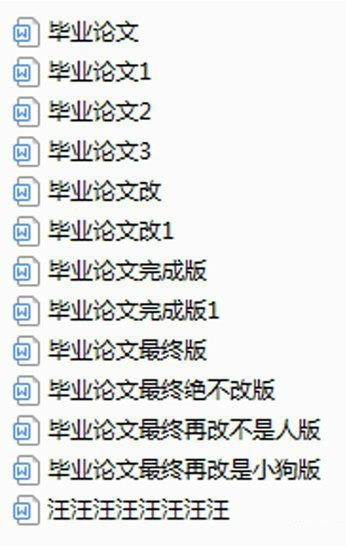
\includegraphics[width=0.95\columnwidth, right]{author-folder/Kai.Wu/thesis_versions.jpg}
    \end{figure}
\end{newminipage}

读到这里,你如果感兴趣可以做个实验,创建一个文件,里面写上一些内容。然后在其他文件夹新建一个同名文件,写上另一些内容。最后,把它拖过来,覆盖掉前面的文件,这时,试一试自己有没有任何办法找回前面文件的内容。

你可能要问,上面不是说了这么多备份方法吗?是的,这些备份方法主要的作用是防丢失,比如电脑丢失、硬盘损坏,但少有备份能做到防覆盖。比如,实时备份的网盘,你本地把文件错误覆盖了,云端也马上被覆盖了。本地备份硬盘,如果备份频率不高,则还有一线生机,但如果过一段时间再去找,也可能找不到了。

因此,为了你的论文(命根子)安全,完全值得再加一层保险:

\begin{enumerate}
    \item Windows开启系统级的文件历史保护:\url{https://www.asus.com.cn/support/FAQ/1013067/},别忘了一定要把你的论文文件夹添加进去才能生效
    \item mac的TimeMachine(时间机器)备份自带了文件历史功能。参照前面的 \ref{sec.pc_backup} 配置好TM,整个电脑的文件历史就都包括在备份里了。
    \item Linux用户,我相信你们有的是办法。最笨的办法,直接写一个shell脚本,把论文文件夹直接复制到其他目录、用日期命名,最后把这个脚本加到crontab里定期运行即可。
    \item 以上是开启本地文件历史的方法。一些网盘自带文件版本功能,但一般限制版本数量或者日期,或者必须要买会员才能开启文件版本。开启过后,相当于云端也存了一份版本历史,万一本地的你没设置好或者其他什么原因不能用,还能在错误覆盖的时候救你一命。学校的seadrive自带大概两个月的文件版本,免费,非常良心,再次建议大家使用。直接把文件夹拖进去备份,就会自动产生文件版本。参见章节 \ref{sec.net_drive_backup} 。
    \item 会一点Git、GitHub的同学,请直接把整个论文文件夹创建成Git项目,并上传到GitHub做成private repo,每天工作结束后交一个commit来备份版本,同时记录你修改了什么内容。对于论文,Git是最完美的备份方案,可以轻松回滚到老版本同时从不担心覆盖、甚至能轻松知道哪个地方的修改是在什么时候引入的,比以上所有方法都靠谱。Overleaf也有GitHub集成,可以方便的与导师协作。但Git学习成本略高,不过网上有无数详尽的教程,感兴趣、学有余力的同学可自行学习。
\end{enumerate}


\begin{flushright}
(2022年12月02日 by Kai Wu)

(major update: 2022年12月30日 by Kai Wu)
\end{flushright}

% \begin{figure}[H]
%     \centering
%     \includegraphics[width=0.5\columnwidth]{author-folder/Kai.Wu/}
% \end{figure}


% \usepackage[export]{adjustbox}

% \item 
% \begin{minipage}{0.3\textwidth}
%     文字
% \end{minipage}
% \begin{minipage}{0.63\textwidth}
%     \begin{figure}[H]
%         \includegraphics[width=0.95\columnwidth, right]{author-folder/Kai.Wu/}
%     \end{figure}
% \end{minipage}

% \input{author-folder/Kai.Wu/.tex}
